\section{Overview}
KUKA.Sim Pro is used for the complete offline programming of KUKA robots. This product allows the analysis of cycle times and the generation of robot programs. It also enables a real-time connection to the virtual KUKA robot controller (KUKA.OfficeLite). KUKA.Sim Pro is additionally used for building parametric components and defining kinematic systems, which can also be used in KUKA.Sim Layout and KUKA.Sim Tech. KUKA.OfficeLite is included in the KUKA.Sim Pro package. CAD importers are available as an option. This requires a purchasable license for each import interface. 
\begin{figure}[h]
\centering
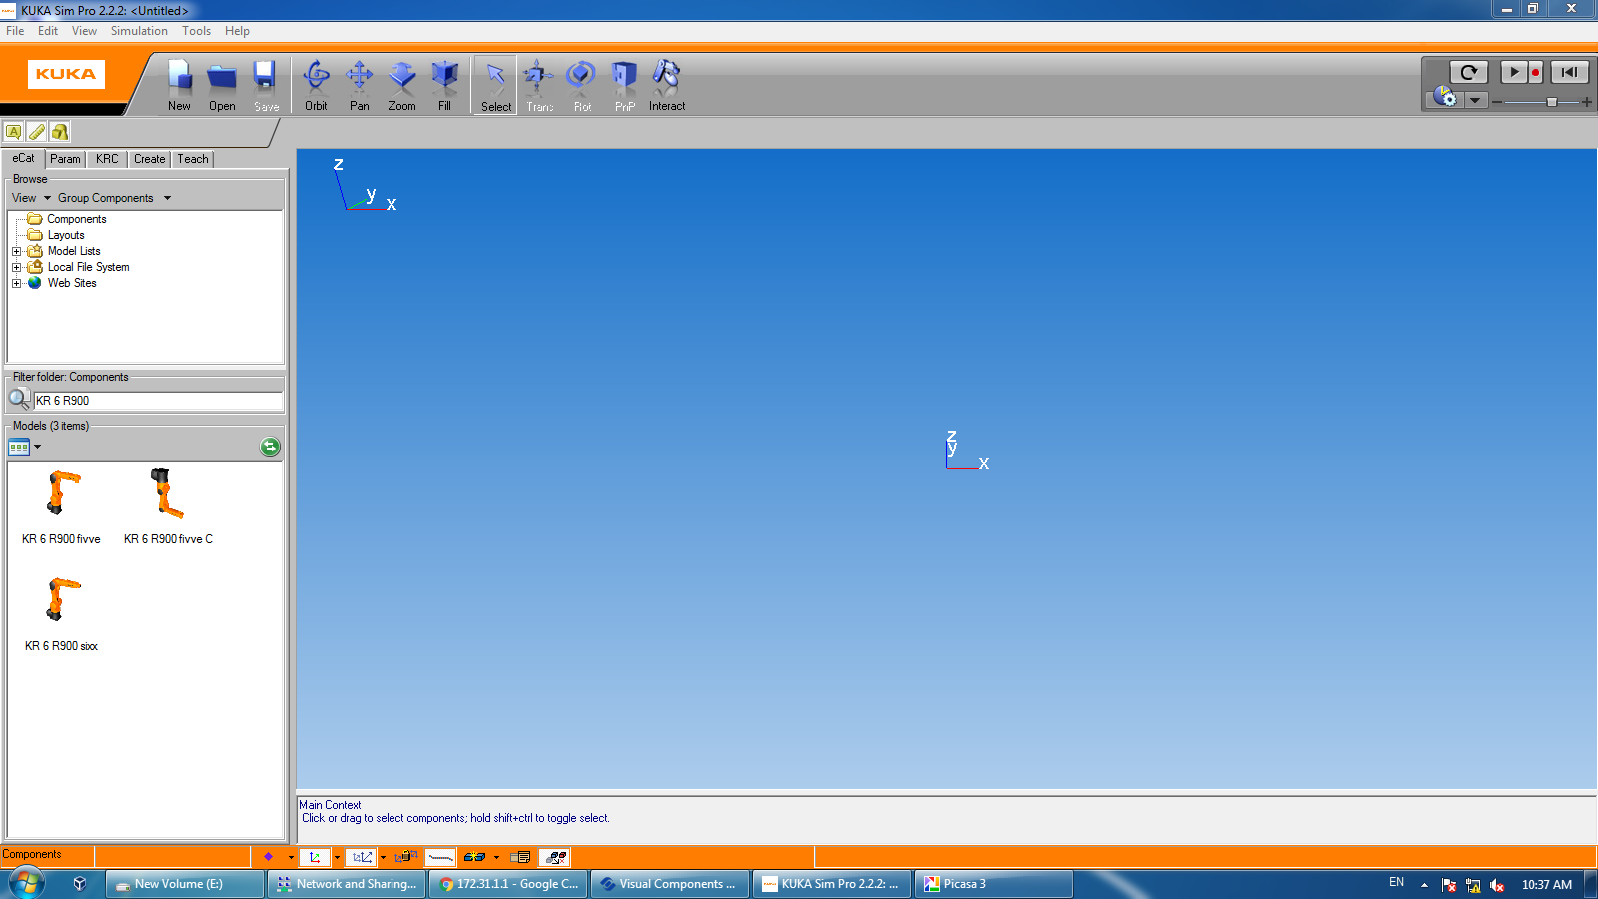
\includegraphics[width=0.9\textwidth]{figures/parts/33}
\label{fig:33}
\caption{KUKA.Sim Pro}
\end{figure}

\section{Requirements}
\begin{itemize}
	\item The minimum requirements for the computer are a 2 GHz CPU and 2 GB RAM, and an OpenGL capable graphics card with at least 512 MB RAM and a resolution of $1024 \times 768$ pixels or a similarly specified notebook.
	\item Supported operating systems are WIN XP - 32-bit or WIN 7 - 32/64-bit.
\end{itemize}

\section{Installaion}
Detailed installation steps can be found in the manual (KUKA.Sim 2.2 - Installation-en), starting page 9. 

\section{License Types}
There are different types of licensing for the KUKA software. License types are determined and verified in accordance with the purchase made from KUKA Roboter GmbH. 
The software licensing concerning the KUKA arm at Zagazig university is an educational bundle license. The serial number for the license is found in the booklet of the KUKA.Sim Pro CD. Information about different licensing bundles are obtained by contacting KUKA Roboter GmbH by email
\url{simulation@kuka-roboter.de.}
Further details about the steps of obtaining the serial key, for different commercial bundles,  are found on page 13 of (KUKA.Sim 2.2- Installation-en) manual.
\begin{mytheo}
 The serial number associated with this purchase is: \texttt {K5P22-N174H-AW7KY-9}
\end{mytheo}

\subsection{Stand-alone License}
The license is on the PC on which KUKA.Sim is used. The license key is then valid for this PC only. It can also be transferred to a different PC, but cannot be used on a two different PCs at the same time, or when either of the two PCs is off.

\subsection{Network License}
Network licenses provide a flexible way of using KUKA.Sim on more than one PC. When a license is requested by a PC, this license is then allocated to this PC. When KUKA.Sim is closed, the license becomes available again and can be accessed by other PCs. 
A license server is required to manage the network licenses. When KUKA.Sim Pro is started, the computer’s identity (IP address, please refer to \textbf {LAN connection} in manual Section “WorkVisual \& LAN connection”) is required occasionally, however, KUKA.Sim Pro needs to check with the local license server to make sure that KUKA.Sim Pro and server are on the same PC, which is required in the network license configuration.

\subsubsection{Installing the license server}
\begin{itemize}
\item Requirements:
“Microsoft Management Console” (MMC) must be installed on the license server. The software can be downloaded from the Microsoft website. In addition, “.NET framework 3.5” or higher should be installed. 
\end{itemize}
After following the installation steps, specified on page 17 of the \textbf {(KUKA.Sim
\textunderscore 2.2\textunderscore Installation\textunderscore en)}manual, there are a few steps required for activation of the serial number for the PC-Robot network.

For network licensing, an account linked with the purchase is created on the Visual Components website \url{http://www.visualcomponents.com/}. In the specified Customer portal \url{https://portal.visualcomponents.net/website/Login.aspx} sign in with the email \url{hodaeltahawy@gmail.com} and password \texttt{quails@123}.

In \textbf{My Products keys} tab, you will find the product key for KUKA.Sim Pro on the KUKA-PC device, at the Mechatronics lab. The license \textbf {is already activated} and will only require renewal after a period of 400 days starting 3-12-2016, which is on \textcolor{red}{7-1-2018}. 

\subsubsection{Manual Licensing}
Manual licensing is performed in case there was no internet connection available. All details about manual licensing in mentioned on page 21 of the (KUKA.Si\textunderscore 2.2
\textunderscore Installation\textunderscore en) manual. 

\textbf {Steps:}
\begin{enumerate}
\item Start the installation of KUKA.Sim Pro 
\item Enter the license key
\item Select “Activate manually” and save the request file
\item Go to the Visual components customer portal and use the given email and password, mentioned in the previous section, to login.
\item On the website, choose Manual Licensing, upload the request file and confirm.
\begin{figure}[h]
\centering
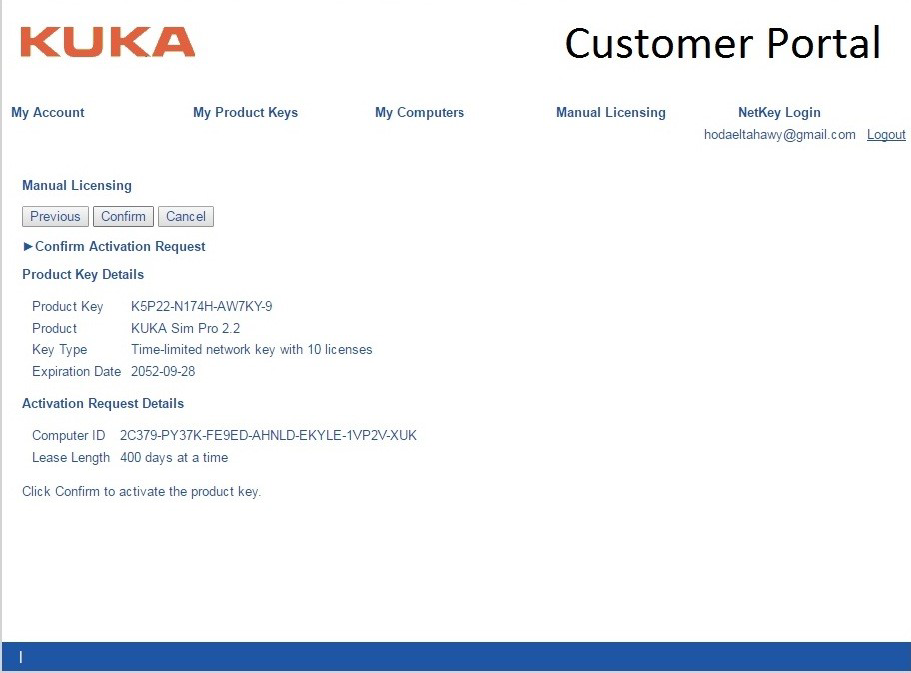
\includegraphics[width=0.9\textwidth]{figures/parts/44}
\label{fig:44}
\caption{Kuka Customer portal}
\end{figure}

\item The license should be activated
\item Download the license (.dat) file and click Finish. 
\item The license (.dat) file should be loaded into the license server, not the KUKA.Sim Pro interface, in order to complete the activation process.
\item After this process is completed, the network server interface should appear as shown in Figure.\ref{fig:55}
    \begin{figure}[h]
        \centering
        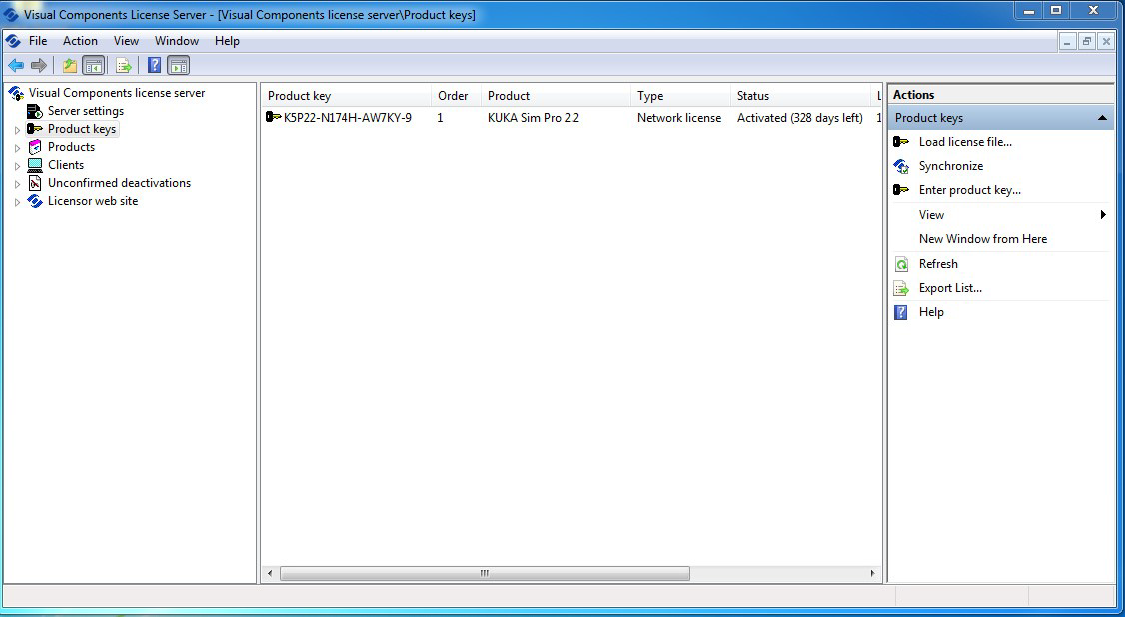
\includegraphics[width=0.9\textwidth]{figures/parts/55}
        \label{fig:55}
        \caption{Kuka network license server interface}
    \end{figure}
\end{enumerate}